\chapter{METODOLOGIA}

\section{Matlab}

MATLAB é um software interativo para computação numérica que possui uma série
de ferramentas, funções, visualisadores, ferramentas para debugging, estrutura de dados, 
entre outros auxilios que facilitam o desenvolvimento e o estudo de atividades
que utilizam a computação numérica. Por conta desses facilitadores, o MATLAB é
amplamente utilizado na indústria e no meio acadêmico.\cite{higham16}
Dada essa característica e a existência da função FMINCON a disposição
no ambiente MATBLAB, foi feita a escolha de se utiliza-lo para
a construção do código presente neste trabalho.

\subsection{fmincon}
Como o modelo matemático a ser otimizado é multivariável e 
possuindo restrições não-lineares, a função FMINCON do ambiente 
do MATLAB é utilizada para otimizar as variações de velocidade 
de forma a diminuir o erro de trajetória associado às 
flexibilidades do sistema que causam perturbações e vibrações 
indesejadas.
É uma função baseada em gradientes que busca por todos os 
mínimos locais de uma região que satisfaz outras restrições 
estipuladas \cite{albaghdadi21}.
Ela utiliza um conjunto de restrições superiores e inferiores 
para cada ponto e otimiza a função considerando as restrições 
estabelecidas pela função não linear, utilizando as equações de 
movimento para encontrar a solução da EDO de maneira a 
otimizar os parâmetros. Também permite uma série de configurações
incluindo a escolha de diferentes algorítimos de otimização entre
outros parâmetros sobre a função.

\section{Geração de Comando}

\subsection{Leitura Gcode}

Foi considerado no mapeamento do Gcode apenas comandos G1, extraindo
as informações dos eixos X, Y e do \textit{feedrate} (F). Com base nesses valores
uma matriz 3 por n é criada, n sendo o número de comandos lidos do arquivo Gcode.
Em geral a unidade de F em arquivos Gcode gerados pelos fatiadores se dão em milímetros por minuto,
mas é convertida para milímetros por segundo na construção da matriz de entrada.

\subsection{Velocidade de curva}

Por conta de alguns problemas de implementação de algoritmos de \textit{lookahead}, a velocidade
de junção, ou seja, a velocidade de transição desejada entre um movimento e outro, foi fixada como 0.
Essa condição representa bem trajetórias que possuem angulos entre os vetores de velocidade dos movimentos
maiores ou iguais a 90°. Portanto, limitando os trajetos testados a esse tipo de trajetória o comando gerado
se manteria próximo da realidade das impressoras 3D.

\subsection{Curva rapezoidal de velocidade}
A partir da matriz de entrada e das velocidades finais e iniciais dos movimentos estabelecida pelo \textit{lookahead},
nos casos apresentados neste trabalho fixadas amabas em zero,
utilizamos a função responsável por gerar a curva trapezoidal de velocidades.

Essa função separa o deslocamento total do movimento em 3 fases de aceleração constante.
Na primeira fase a velocidade trazida da velocidade incial até a velocidade desejada
a aceleração constante, na segunda fase a velocidade é mantida constante na velocidade desejada
e por fim na terceira fase a velocidade é levada da velocidade desejada até a velocidade final.
Entretanto, em algumas situações pode não ser possível alcançar a velocidade desejada
e o perfil se limitar a duas fases, outras condições onde alguma das velocidades é igual a
velocidade desejada faz com que a quantidade de fases visiveis seja reduzida.

Para identificar se a velocidade desejada será alcançada é calculado a velocidade pico ($v_p$)
que é obtida extrapolando retas com as inclinações da aceleração na velocidade incial e final.
É possível obter a velocidade de pico através da equação \ref{eq:v_p}.

\begin{equation}
    \label{eq:v_p}
    v_p = \sqrt{\frac{(v_i^2+v_f^2)}{2}+acc*des_{tot}}
\end{equation}

A partir da comparação da velocidade pico com a velocidade desejada, indicada pelo \textit{feedrate} disponibilizado no Gcode,
é possível determinar o padrão da curva de velocidade deste movimento.
Caso a velocidade de pico for maior do que a velocidade desejada, temos 3 fases de deslocamento
que podem ser calculadas pelas equações \ref{eq:des_seg_acc} e \ref{eq:des_seg_no_acc}.
Caso a velocidade de pico seja igual ou menor do que a velocidade desejada, teremos 2 fases de deslocamento
que são calculadas a partir da equação \ref{eq:des_seg_acc}.

\begin{equation}
    \label{eq:des_seg_acc}
    des_{segment} = \frac{(v_f^2-v_i^2)}{(2*acc_{segment})}
\end{equation}

\begin{equation}
    \label{eq:des_seg_no_acc}
    des_{middle} = des_{total}-(des_{up}+des_{down})
\end{equation}

É possível calcular também os intervalos de tempo dessas fases, através das 
equações \ref{eq:dt_seg_acc} e \ref{eq:dt_seg_no_acc}.

\begin{equation}
    \label{eq:dt_seg_acc}
    dt_{segment} = \frac{(v_f-v_i)}{acc_{segment}}
\end{equation}

\begin{equation}
    \label{eq:dt_seg_no_acc}
    dt_d = \frac{des_d}{v_d}
\end{equation}

Além disso é calculado a variação de velocidade nos intervalos pela equação \ref{eq:delta_vel}.

\begin{equation}
    \label{eq:delta_vel}
    \Delta vel = v_f-v_i
\end{equation}

Esses passos resultam em uma nova matriz contendo informações
sobre o a variação da posição, do tempo, da velocidade e sobre a aceleração e 
direção de deslocamento nos pontos iniciais e finais do Gcode e também nos pontos
onde existe uma alteração na aceleração.

\subsection{Interpolação}

A partir dessa matriz, é utilizada uma função de interpolação para dividir cada intervalo dessa matriz em intervalos menores
baseados em um passo de tempo definido para esta interpolação.
Assim criando-se uma nova matriz dos dados interpolados.
Para se dividir esses intervalos é possível utilizar a equação \ref{eq:N_steps}
calculando o número de passos neste intervalo, anexando à matriz os passos de tempo e por fim
o restante do intervalo, calculado pela equação \ref{eq:dt_interpol_last_step}.
Com base nestes passos de tempo, é possível calcular o deslocamento para cada um destes passos
através da equação \ref{eq:delta_des_interpol}.

\begin{equation}
    \label{eq:N_steps}
    N_{steps} = \lceil\frac{\Delta t_i}{\Delta t_{step_{size}}}-1\rceil
\end{equation}

\begin{equation}
    \label{eq:dt_interpol_last_step}
    \Delta t_{last_{step}}= \Delta t_i - \Delta t_{step_{size}}*N_{steps} 
\end{equation}

\begin{equation}
    \label{eq:delta_des_interpol}
    \Delta des_i = \Delta v_i*\Delta t_i+ \frac{acc_{segment}*\Delta t_i^2}{2} 
\end{equation}

A partir dos vetores de direção e da função acumuladora que se consite em acumular os valores de um vetor.
Obtemos uma matriz de posições, velocidades e tempo.

\begin{equation}
    \label{eq:acumulator_function}
    \begin{split}
        v_{0} &= init_{value} + v_{0} \\
        v_k &= v_k+v_{k-1}
    \end{split}
\end{equation}

\section{Modelagem dinâmica de uma impressora 3D}
Para a modelagem do sistema mecânico são consideradas as seguintes simplificações:
\begin{itemize}
    \item Não existe escorregamento nem perda de potência na interação entre a polia e a correia
    \item A correia apresenta um comportamento equivalente à uma mola e um amortecedor em paralelo
    \item O bico injetor é um corpo rígido uniforme de geometria simples
    \item A correia está acoplada nos dois lados da peça que se movimenta nos trilhos, entretanto como a correia só permite o tensionamento ela será considerada como um conjunto mola amortecedor simples
\end{itemize}

Para a modelagem dinâmica dos eixos X e Y da impressora 3D, 
é considerado que os eixos são completamente independentes, 
a flexibilidade da correia é aproximada utilizando um conjunto 
mola amortecedor e a transmissão de movimento e torque dos 
motores é considerada como ideal e não será abordada.
Assim duas posições de estudo surgem para cada eixo, uma delas 
representa a posição ideal, caso o sistema não possuiesse nenhuma flexibilidade
ou perda, que também é a posição desejada pelo usuário ($px_b$). 
A segunda posição considera as forças inerciais e a 
flexibilidade introduzida pela correia, ou seja, a posição real simulada pelo modelo
e no caso empírico a posição real ($px$) como na figura \ref{fig:din_model}.


\begin{figure}[!htb]
    \centering
    \caption{Visualização das posições do sistema}
    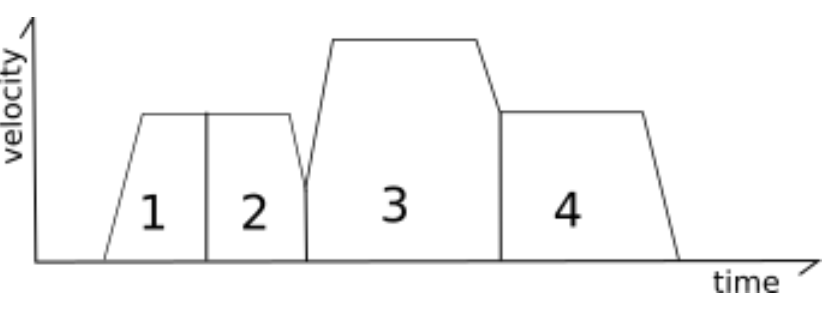
\includegraphics[scale=0.4]{trapezoidex}

    \label{fig:din_model}
\end{figure}

\begin{multline}
    \label{eq:mov_impressora}
    m \ddot{px} + c(\dot{px} - \dot{px_b}) + k(px-px_b) = 0 \\
    \ddot{px}  = - \frac{c}{m}(\dot{px} - \dot{px_b}) - \frac{k}{m}(px-px_b) \\
    \ddot{px}  = - \frac{c}{m} \dot{px} + \frac{c}{m} \dot
    {px_b} - \frac{k}{m} px + \frac{k}{m} px_b \\
    \ddot{px}  = - \frac{c}{m} \dot{px} - \frac{k}{m} px + \frac{c}{m} \dot{px_b} + \frac{k}{m} px_b
\end{multline}

\subsection{Espaço de estados}
A formulação de espaço de estados foi utilizada com intuito de facilitar as operações e
a a solução do sistema, dado sua característica de dividir uma equação diferencial
de ordem superior em um sistema de equações diferenciais de ordem 1.
O modelo dinâmico do sistema é apresentado na formulação de espaço de estados 
na equação \ref{eq:espaco_de_estados_din_model}, baseado na equação \ref{eq:mov_impressora},
utilizando a mesma equação para a base do eixo y.

\begin{equation}
    \label{eq:espaco_de_estados_din_model}
    \begin{bmatrix}
        \dot{px} \\
        \ddot{px} \\
        \dot{py} \\
        \ddot{py}
    \end{bmatrix}
    =
    \begin{bmatrix}
        0 & 1 & 0 & 0 \\
        -\frac{k_x}{m_x} & -\frac{c_x}{m_x} & 0 & 0 \\
        0 & 0 & 0 & 1 \\
        0 & 0 & -\frac{k_x}{m_x} & -\frac{c_x}{m_x}
    \end{bmatrix}
    \begin{bmatrix}
        px \\
        \dot{px} \\        
        py \\
        \dot{py} \\
    \end{bmatrix}
    +
    \begin{bmatrix}
        0 & 0 & 0 & 0 \\
        \frac{k_x}{m_x} & \frac{c_x}{m_x} & 0 & 0 \\
        0 & 0 & 0 & 0 \\
        0 & 0 & \frac{k_x}{m_x} & \frac{c_x}{m_x}
    \end{bmatrix}
    \begin{bmatrix}
        px_b \\
        \dot{px_b}  \\
        py_b \\
        \dot{py_b} 
    \end{bmatrix}
\end{equation}

Em uma notação simplificada temos a equação \ref{eq:simp_state_space_din_model}
\begin{equation}
    \label{eq:simp_state_space_din_model}
    \dot x = A*x+B*u
\end{equation}

\section{FMINCON}

\subsection{Configurações da função}
Foi utilizado o seguinte conjunto de configurações opcionais da função (tabela \ref{tab:fmincon_options}).
As configurações não indicadas se mantem na configuração padrão, que pode ser encontrada nos manuais da mesma.

\begin{table}
    \begin{center}
    \caption{Tabela de parâmetros opcionais da FMINCON}
    \label{tab:fmincon_options}
    \begin{tabular}{c c}
        Opção & Valor \\ \hline
        TolFun & 0.000000001 \\
        MaxIter & 100000 \\
        Display & iter \\
        DiffMinChange & 0.0001 \\
        Algorithm & interior-point \\
        StepTolerance & 1e-12 \\
        MaxFunEvals & 700000  \\ \hline
    \end{tabular}
    \end{center}
\end{table}

\subsection{Restrições lineares e limites de borda}
Não foi utilizado nenhuma restrição linear nessa otimização.
Os limites superiores (\textit{upperbound}) e inferiores (\textit{lowerbound}) foram definidos
baseados nos limites físicos da impressora (0 a 200 milímetros) para as posições $x_b$ e $y_b$.

\subsection{Restrições não lineares}
A função para as restrições não lineares foi implementada com base nas equaqções \ref{eq:state_center_segment},
\ref{eq:state_dot_center_segment}, \ref{eq:defect_calc}, \ref{eq:input_value_center_segment} de maneira a
popular a variável de restrições de igualdades com os valores do defeito dos segmentos ($\Delta$) e também
com os valores iniciais. 
Além disso, foi utilizado também como restrição de equalidade a arrancada, atrelado a um condicional para que
se comporte como uma inequalidade.
A variável de restrições de inequalidades não foi populada, os motivos são apresentados
na seção de resultados e discussão.

\subsection{Função objetivo}
Foram realizados alguns testes com funções objetivo e seus resultaods são apresentados na seção de resultados e discussão,
entretanto a função objetiva foi definida como zero, ou seja, pra qualquer valor ela retornara zero nas chamadas da FMINCON.

\section{Solução da trajetória da base}

É considerada como trajetória desejada a trajetória obtida através da função de geração de comando apresentada anteriormente
e são utilizados os vetores de tempo e posição como variáveis globais, para serem acessados dentro da função das
restrições não lineares, chamada pela FMINCON.
Além disso, esses mesmos vetores de posição também são considerados como o chute inicial e variável principal
na FMINCON, sendo adaptados em forma de matriz.

A variável principal inserida na FMINCON é a matriz contendo os vetores de posição da base ($x_b$ e $y_b$),
enquanto os vetores de posição da ponta é fixado pela trajetória desejada presente na forma de variáveis globais.

Para conseguir realizar os cálculos necessários dentro da função de restrições não lineares é utilizado o seguinte conjunto
de equações basicas (\ref{eq:der_acc}) para se derivar a curva posição-tempo considerando aceleração constante,
sendo $dt$ a variação do tempo no intervalo, $des_n$ o deslocamento final do intervalo, $des_i$ o deslocamento inicial no intervalo,
$acc_n$ a aceleração do intervalo, $vel_n$ a velocidade final do intervalo e $vel_i$ a velocidade inicial do intervalo.
Assim construindo o vetor de velocidade a partir da condição inicial de deslocamento e velocidade zero, para ambos os eixos ($x$ e $y$).

\begin{equation}
    \label{eq:der_acc}
    \begin{split}        
        acc_n = 2\frac{(\frac{des_n-des_i}{dt})-vel_i)}{dt} \\
        vel_n = vel_i+acc_ndt \\
    \end{split}
\end{equation}

\section{Descrição das simulações}

Variação da frequência
range (50 a 500) rad/s
Variação do coeficiente de amortecimento
range (0 a 2) delta variado

Variação da velocidade desejada
range (20 a 200)mm/s

Variação da aceleração máxima
range (1000 a 10000)mm/s²

Variação da resolução de dt
range (0.01 a 0.0002)s


tempo de simulação
tamanho dos vetores
Parametors fmincon Viabilidade, passo minimo
omega_d
k
b

Curvas